\documentclass[openany]{article}

%Standard Stefanos Packages
\usepackage[utf8]{inputenc}
\usepackage{dirtytalk}
\usepackage{amsmath}
\usepackage{mathtools}  
\mathtoolsset{showonlyrefs} 
\usepackage{graphicx}
\usepackage{mdframed}
\usepackage{lipsum}
\usepackage{cancel}
\usepackage{systeme}
\usepackage{pgfplots}
\usepackage{textcomp}
\usepackage{geometry}
\usetikzlibrary{arrows}
\geometry{a4paper}
\graphicspath{ {./res/} }
\usepackage{float}
\restylefloat{table}
\newcommand{\comment}[1]{%
	\text{\phantom{(#1)}} \tag{#1}
}
\title{\line(3,0){250}\\PROGRAMMING IN PYTHON FOR DATA SCIENCE(CS3PP19) \\ Final Exam: Question 3  \\\line(3,0){250}}
\usepackage{pgfplots}
\author{52944}
\newmdtheoremenv{note}{Note}
\pgfplotsset{compat=1.17}


%Extra Packages
\usepackage{tikz}
\usetikzlibrary{automata,positioning}

\usepackage{listings}
\usepackage{xcolor}

\definecolor{dkgreen}{rgb}{0,0.6,0}
\definecolor{gray}{rgb}{0.5,0.5,0.5}
\definecolor{mauve}{rgb}{0.58,0,0.82}

\lstdefinestyle{myScalastyle}{
	frame=tb,
	language=scala,
	aboveskip=3mm,
	belowskip=3mm,
	showstringspaces=false,
	columns=flexible,
	basicstyle={\small\ttfamily},
	numbers=none,
	numberstyle=\tiny\color{gray},
	keywordstyle=\color{blue},
	commentstyle=\color{dkgreen},
	stringstyle=\color{mauve},
	frame=single,
	breaklines=true,
	breakatwhitespace=true,
	tabsize=3,
}

\begin{document}
	\maketitle
	\section{Initialization Code}
		\begin{lstlisting}[language=Python]
import pandas as pd
import seaborn as sns
data = pd.read_csv("data.csv")
data=data.dropna()
data
		\end{lstlisting}
	\section{Q3.a.i}
		Trying to answer this question directly, will lead to misleading results. 
		\begin{lstlisting}[language=Python]
#Creating category as cartesian product of school-gender
ms_male=data.loc[(data.school=="MS") & (data.sex=="M")].reset_index()
ms_female=data.loc[(data.school=="MS") & (data.sex=="F")].reset_index()
gp_male=data.loc[(data.school=="GP") & (data.sex=="M")].reset_index()
gp_female=data.loc[(data.school=="GP") & (data.sex=="F")].reset_index()
#Creating the new categorical variable
ms_male["school_gender"]="MS-M"
ms_female["school_gender"]="MS-F"
gp_male["school_gender"]="GP-M"
gp_female["school_gender"]="GP-F"
#Concatenate the datasets
data=pd.concat([ms_male,ms_female,gp_male,gp_female])
#plot
sns.countplot(x="school_gender",hue='grade',data=data)
		\end{lstlisting}
		\begin{figure}[H]
			\iftrue
			\centering
			\caption{Distribution of grades by school and gender}
			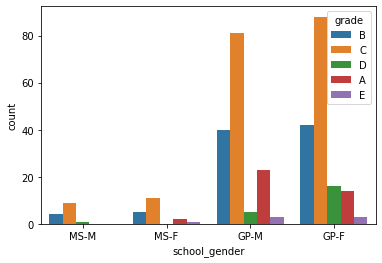
\includegraphics[scale=0.5]{q3-a-i-1}
			\fi
		\end{figure}
		Thats because the dataset is severily undersampled, on the school categorical data, for the value MS. running a count query reveals the issue
		\begin{lstlisting}[language=Python]
"""
This dataset has issue. MS School is undersampled. 
"""
data.groupby("school").school.count()
		\end{lstlisting}
		\begin{table}[H]
			\centering
			\begin{tabular}{ll}
				GP  & MS \\
				315 & 35
			\end{tabular}
		\end{table}
		We can bypass this by sampling the oversampled class, in this case, GP class is oversampled with 315 samples. 
		\begin{lstlisting}[language=Python]
ms=data.loc[data.school=="MS"]
gp=data.loc[data.school=="GP"]
sampled_gp=gp.sample(35)

sampled_balanced_data=pd.concat([ms,sampled_gp]).reset_index()
data=sampled_balanced_data
		\end{lstlisting}
		Now, we have a set of equal classes.
		\begin{figure}[H]
			\iftrue
			\centering
			\caption{Distribution of grades by school and gender, sampled}
			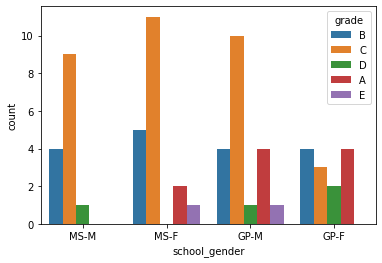
\includegraphics[scale=0.5]{q3-a-i-2}
			\fi
		\end{figure}
		Of course this is not a perfect solution, as we loose prestision over the oversampled class. This techique should always used with care.
		Please note that the above task could also be achieved with the following statement
		\begin{lstlisting}[language=Python]
x=data.groupby(['school','grade','sex']).sex.count().plot.bar()
		\end{lstlisting}
		with the following end-result
		\begin{figure}[H]
			\iftrue
			\centering
			\caption{Distribution of grades by school and gender, sampled}
			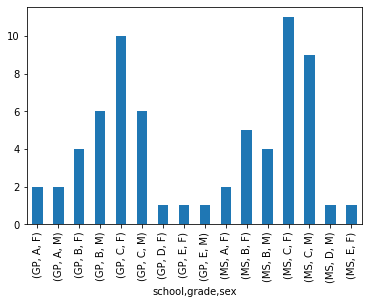
\includegraphics[scale=0.5]{q3-a-i-3}
			\fi
		\end{figure}
		
	\section{Q3.a.ii}
		\begin{lstlisting}[language=Python]
#select rows for creating sudo-category
grade_ab=data.loc[(data.grade=="A") | (data.grade=="B")]
grade_cd=data.loc[(data.grade=="C") | (data.grade=="D")]
grade_e=data.loc[(data.grade=="E")]
#create sudo category
grade_ab["grade_category"]="AB"
grade_cd["grade_category"]="CD"
grade_e["grade_category"]="E"
#concat the dataset again
data=pd.concat([grade_ab,grade_cd,grade_e])
#find the mean . grouby the sudo category
average_study_time=data.groupby("grade_category").studytime.mean()
		\end{lstlisting}
		\begin{table}[H]
			\centering
			\begin{tabular}{lll}
				A-B      & C-D      & E        \\
				2.428571 & 1.863636 & 1.000000 \\
			\end{tabular}
		\end{table}
		This is misleading though, as the categories A-B and E are undersampled. We can verify this by typing...
		\begin{lstlisting}[language=Python]
data.groupby("grade_category").grade_category.count()
		\end{lstlisting}
		\begin{table}[H]
			\centering
			\begin{tabular}{lll}
				A-B      & C-D      & E        \\
				21 & 44 & 1 \\
			\end{tabular}
		\end{table}
		Therefore, we need to discard E from our analysis, as nothing can be done for this category(we cant sample every category to 1 point only!) 
		Depending on our needs for accuracy, we may need to downsample the category C-D, but for the purposes of this ECD, as well as the query given, 
		i consider this unessesary.
	\section{Q3.a.iii}
		Lets create the nessesary plots, for the family size vs grade, this can be done easily...
		\begin{lstlisting}[language=Python]
data.groupby(['famsize','grade']).count()["index"].plot.bar()
		\end{lstlisting}	
		\begin{figure}[H]
			\iftrue
			\centering
			\caption{Family size vs Grades}
			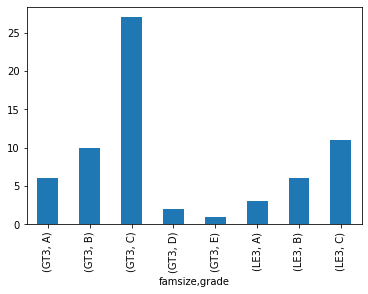
\includegraphics[scale=0.5]{q3-a-ii-1}
			\fi
		\end{figure}
		parental education though, is sligly more complicated, as i need to define what 'parential education' is . I did that with the following metric
		\begin{equation}
			Pedu=\frac{Medu+Fedu}{8}
		\end{equation}
		Lets then apply this row transformation to our dataset
		\begin{lstlisting}[language=Python]
data['Pedu'] = data.apply(lambda x: ((x["Medu"]+ x["Fedu"])/8,axis=1)
		\end{lstlisting}	
		From now on, creating a boxplot is straightforward
		\begin{lstlisting}[language=Python]

datapoints = []
labels=data['grade'].unique()
for c in labels:
	datapoints.append(data.loc[data.grade==c,'Pedu'])
plt.boxplot(datapoints,labels=labels)
display
		\end{lstlisting}
		\begin{figure}[H]
			\iftrue
			\centering
			\caption{Parental education vs Grades}
			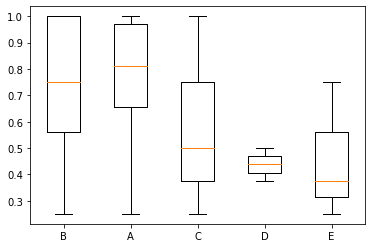
\includegraphics[scale=0.5]{q3-a-ii-2}
			\fi
		\end{figure}
		As we can see clearly in the respective boxplot and barchart, the parental education influences the grades of the children.
	\section{Q3.a.iv}
		In order to answer this question, we need to perform the following tasks
		\begin{itemize}
			\item Convert the grade to a \textbf{ordered} numeric variable
			\item Generate the corellation matrix of the data
			\item Pick the 'grade' column
		\end{itemize}
		Lets perform the first step	
		\begin{lstlisting}[language=Python]
mappings={"grade":{"A":5,"B":4,"C":3,"D":2,"E":1}}
data=data.replace(mappings)
		\end{lstlisting}
		Here, we perform a mapping, notice the ordering of the grades. 5 (A) is better than 1 (E).
		Now we should generate the corellation matrix, and pick the grade column
		\begin{lstlisting}[language=Python]
bad_grades = data.corr()["grade"].sort_values()[:3]
good_grades = data.corr()["grade"].sort_values()[-5:-1] #do not pick grade variable
		\end{lstlisting}
		\begin{table}[H]
			\centering
			\caption{3 best features related to bad grades}
			\begin{tabular}{lll}
				
				traveltime & -0.230319 &  \\
				Walc       & -0.221261 &  \\
				absenses   & -0.217952 & 
			\end{tabular}
		\end{table}
		\begin{table}[H]
			\caption{3 best features related to bad grades}
			\centering
			\begin{tabular}{lll}
				studytime & 0.216986 & \\
				Fedu      & 0.349496 & \\
				Medu      & 0.393533 & \\
				Pedu	  & 0.419606 & \\
			\end{tabular}
		\end{table}
		The Pedu metric is included, as a proof of a quality of the metric for the question Q3.a.ii
		
	
\end{document}